\chapter{Gerenciamento do Sistema de Filtragem}
\label{chap:pm}

O capítulo \ref{chap:sistema_filtragem} apresentou toda a complexidade do sistema de filtragem do ATLAS. Como o projeto desenvolvido neste trabalho é para execução dentro deste ambiente, torna-se imperativo ser capaz de colocar toda esta infra-estrutura em operação, para observar como o sistema desenvolvido se comportará durante sua operação nominal. 


\section{O Servidor de Base de Dados}
\label{sec:oks}

Assim, surge a necessidade de prover uma base de dados de configuração que se encarregará de determinar quais módulos estarão ativos, e quais as configurações de cada um, além de prover uma interface para que cada aplicativo acesse seus parâmetros de configuração. Os requisitos de tempo, escalabilidade e arquivamento do sistema de filtragem do ATLAS tornam as aplicações de base de dados comercialmente existentes inviáveis, resultando na necessidade de criar-se uma base de dados própria, capaz de atender a estes requisitos. 

Com esta finalidade, foi desenvolvido a base de dados OKS (\emph{Object Kernel Support}) \cite{bib:oks}. No OKS, cada aplicação ou recurso do sistema de filtragem é descrito como uma classe em uma base de dados de \emph{schema}. Esta base contém a descrição de todas as classes, os atributos disponíveis, relações de herança e dependência com outras classes, etc, de acordo com o conceito de programação orientada a objetos \cite{bib:poo}. Adicionalmente, o OKS fornece um ambiente onde o usuário pode descrever como gostaria de configurar o sistema de filtragem de alto nível, através do instanciamento e configuração de parâmetros das classes contidas no \emph{schema} e, ao final, gerar uma base de dados de configuração. Esta base será, no momento da inicialização do sistema de \emph{trigger}, lida por um aplicativo de controle, que será responsável por inicializar cada um dos aplicativos do sistema de filtragem em seus respectivos nós de processamento. Em seguida, cada aplicação deverá acessar esta base de dados de configuração de forma a configurar parâmetros que digam respeito ao seu funcionamento em especial (tamanho de filas, protocolo de comunicação a ser usado, valores de \emph{timeout}, etc).  

\begin{figure}
\begin{center}
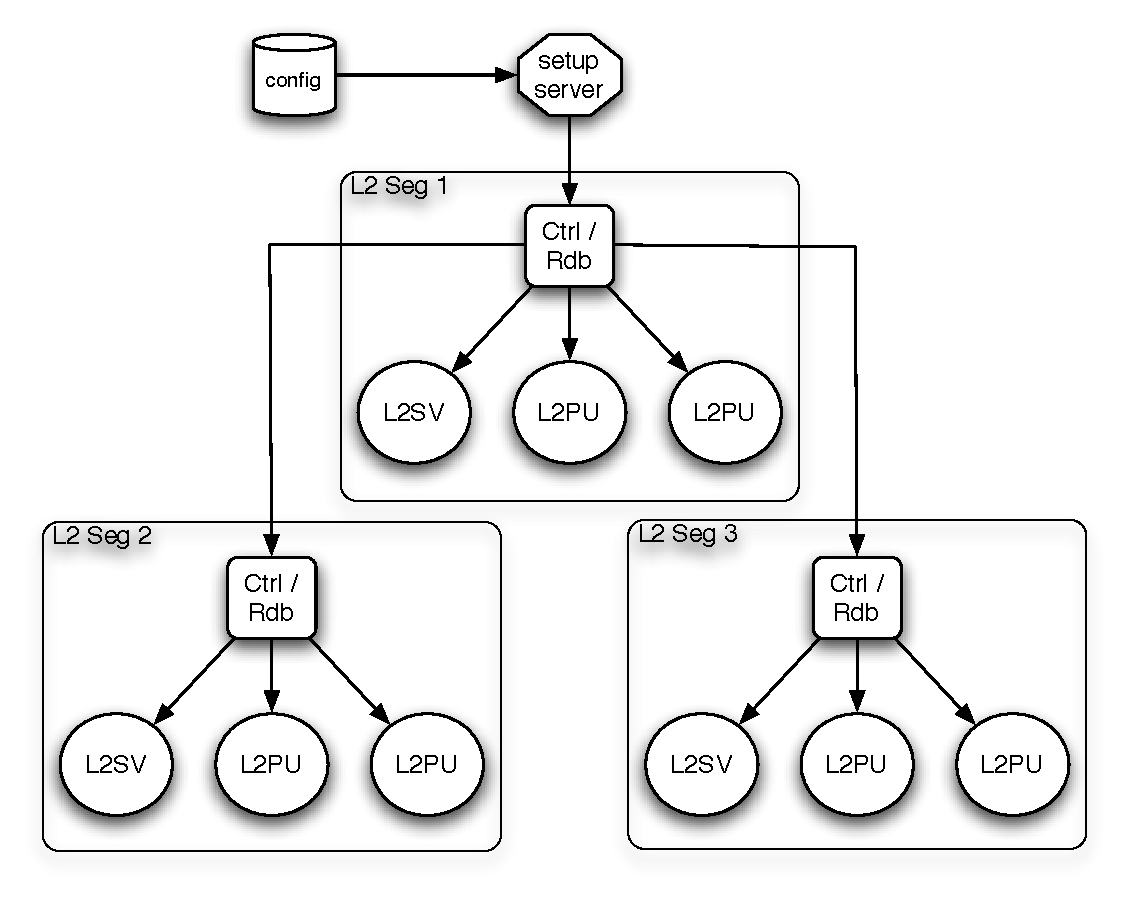
\includegraphics[width=0.6\textwidth]{oks_multi_control_strategy}
\caption{Estrutura de controle hierárquico do sistema de filtragem.}
\label{fig:multi_control}
\end{center}
\end{figure}

Para garantir sua escalabilidade, o sistema de filtragem pode ser dividido, logicamente, em \emph{segmentos}. Cada segmento contém sempre um controlador responsável por gerir os aplicativos dentro daquele segmento. Adicionalmente, utilizam-se múltiplos servidores de configuração, para evitar gargalos durante a fase de configuração. É apresentado, na Fig.~\ref{fig:multi_control}, um exemplo desta abordagem de controle hierárquico através da utilização de múltiplos segmentos. Como se percebe, ao multiplicar-se o número de aplicações de controle, diminui-se a carga de operações em cada controlador, permitindo que o número de aplicações aumente indefinidamente.  

Para a geração da base de dados de configuração, bem como a leitura da mesma, o ambiente OKS oferece interfaces de acesso em C++. Desta forma, o usuário fica isento dos detalhes de implementação e de localização da base de dados (local ou remota). Entretanto, a tarefa de configurar cada objeto, bem como a relação entre eles e sua organização lógica em segmentos, ainda fica a cargo do usuário, o que representa uma tarefa bastante penosa e delicada, requerendo conhecimento especialista, nem sempre disponível.


\section{O \emph{PartitionMaker}}
\label{sec:pm}

No início do desenvolvimento do sistema de filtragem de alto nível, as partições de configuração eram criadas manualmente, visto que a partição é um arquivo texto contendo os objetos descritos em linguagem XML \cite{bib:xml}. Entretanto, esta solução tornou-se rapidamente inviável devido ao grande número de componentes a serem configurados.

A primeira abordagem automática para a criação de base de dados de configuração era baseada em \emph{templates}. Nesta abordagem, o código XML de um objeto de cada classe ficava descrito como um modelo em um arquivo texto. Apenas alguns parâmetros podiam ser configurados, e os demais tinham valores pré-fixados. O usuário era, então, obrigado a configurar todos os parâmetros variáveis, o que restringia a utilização da ferramenta apenas aos usuários experientes. A falta de testes de consistência dos valores configurados resultava em freqüentes execuções mal sucedidas do sistema de filtragem. Por fim, como a descrição de cada objeto estava fixada, qualquer mudança na classe de um dado objeto, ou na implementação da base de dados, inutilizava a ferramenta de configuração até que o desenvolvedor da mesma atualizasse a sua base de \emph{templates}.

\begin{figure}
\begin{center}
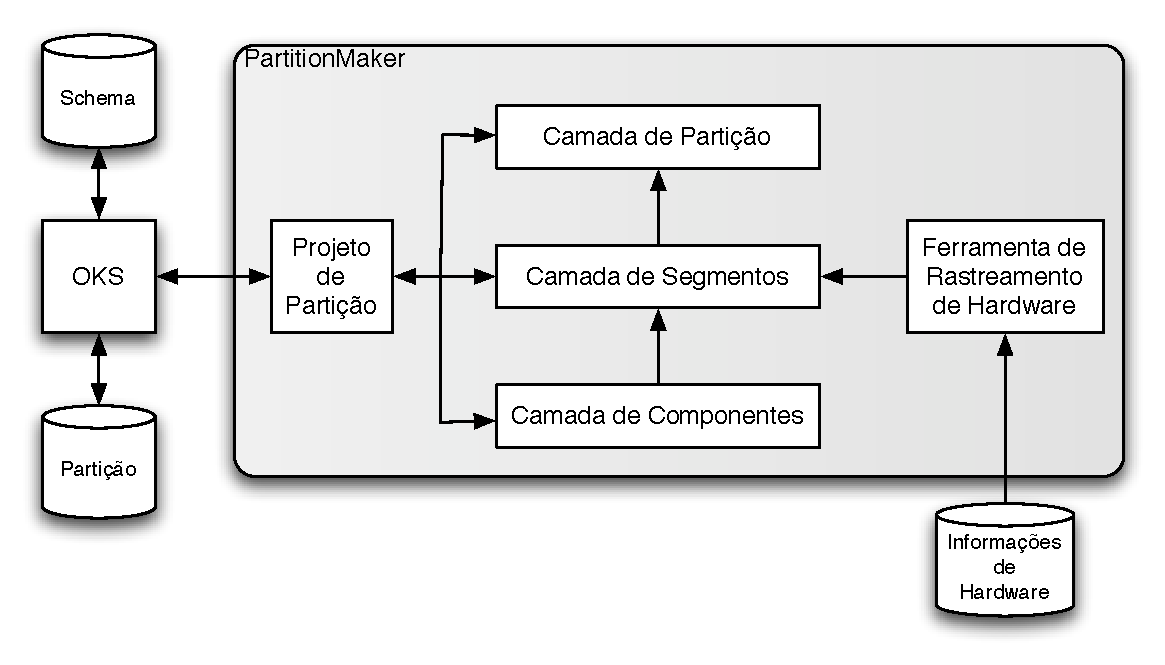
\includegraphics[width=0.65\textwidth]{partitionmaker_block_diagram}
\caption{Diagrama em blocos do \emph{PartitionMaker}.}
\label{fig:pm}
\end{center}
\end{figure}

Para se obter configuração automatizada, superando as falhas observadas nas abordagens anteriores, o \emph{PartitionMaker}, cujo diagrama é apresentado na Fig.~\ref{fig:pm}, foi desenvolvido. A filosofia deste ambiente é agregar o conhecimento especialista a respeito do sistema de filtragem, de forma que os usuários com diferentes níveis de conhecimento sobre o sistema de filtragem possam ser conduzidos com segurança durante o processo de configuração, resultando em execuções otimizadas e minimizando as possibilidades de erros. Por fim, o ambiente deve operar integrado à base de dados OKS, de forma a garantir que mudanças ocorridas na classe de um dado objeto sejam imediatamente reconhecidas pelo \emph{PartitionMaker}.

Ao ser inicializado pelo usuário, o \emph{PartitionMaker} lê a base de dados de \emph{schema} e gera uma representação em \emph{Python} \cite{bib:python} de cada uma das classes existentes. Esta leitura é realizada utilizando \emph{bindings} de C++ para Python \cite{bib:boost}, permitindo que o \emph{PartitionMaker} usufrua dos recursos já implementados na base de dados OKS, além de isentar o \emph{PartitionMaker} dos detalhes de implementação da base de dados de configuração e \emph{schema}. Toda esta operação de comunicação com o OKS é realizada pelo módulo de  \emph{Projeto de Partição}, de forma a abstrair do resto do sistema os detalhes desta comunicação.

\begin{figure}[t]
\begin{center}
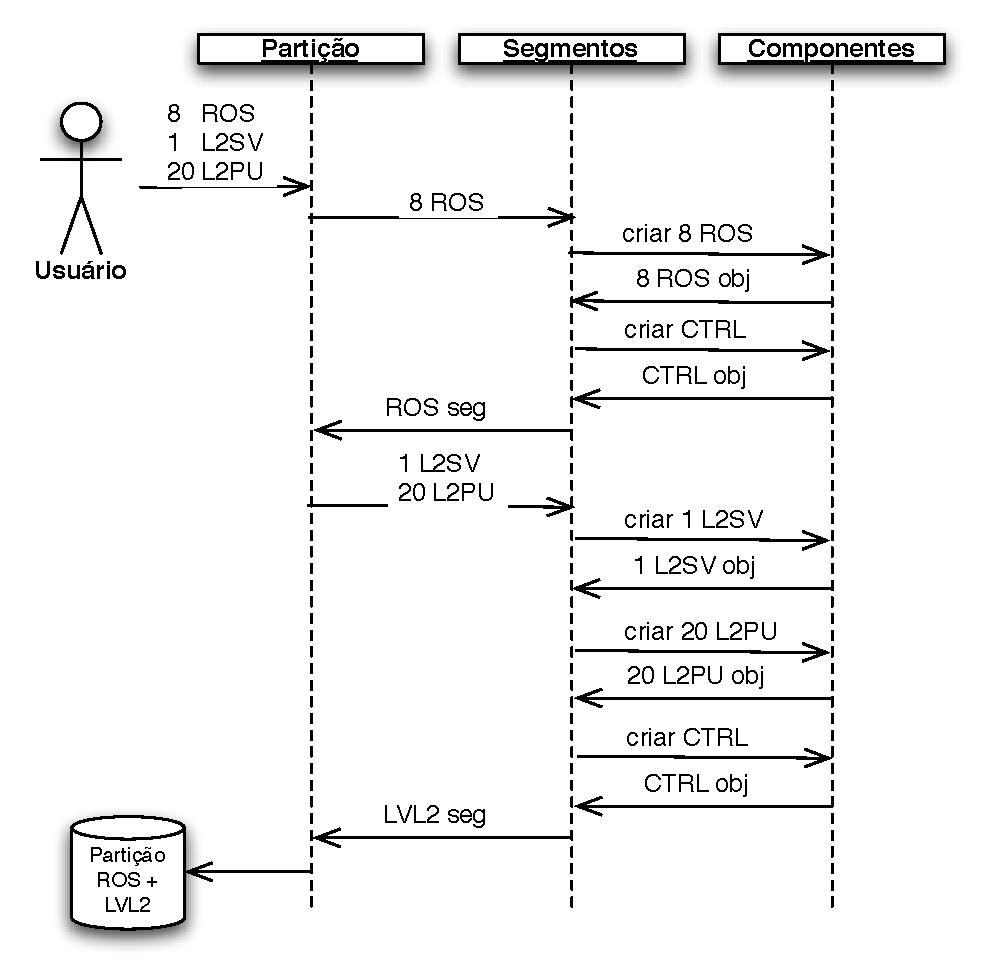
\includegraphics[width=0.6\textwidth]{partitionmaker_generation_flow}
\caption{Exemplo de fluxo de geração de uma partição.}
\label{fig:pm_flow}
\end{center}
\end{figure}

Após a inicialização, o usuário recorre aos diversos módulos e funções disponíveis, para atingir seus objetivos de configuração. De forma a atender uma vasta gama de usuários, com diferentes graus de familiaridade com o sistema de filtragem, uma abordagem em três camadas foi utilizada.

A camada mais baixa (\emph{Camada de Componentes}) é responsável por configurar cada objeto OKS individualmente. O controle de consistência, nesta camada, restringe-se a verificar se os limites aceitáveis para determinados atributos, tipo de dado inserido, entre outros, fazem sentido. Os objetos OKS são criados utilizando-se as funções da  base de dados OKS, evitando a replicação de código.

A segunda camada (\emph{Camada de Segmentos}) responsabiliza-se por acessar os objetos configurados pela primeira e agrupá-los na forma de segmentos com significado lógico para o sistema de filtragem. É de responsabilidade desta camada assegurar que as relações entre as aplicações dentro de um mesmo segmento estejam corretas, e que as aplicações contidas no mesmo apresentam relações entre si (por exemplo, evitando que uma aplicação do filtro de eventos esteja presente em um segmento destinado ao segundo nível). 

A última camada (\emph{Camada de Partição}) se encarrega de agrupar os segmentos gerados em uma base final de configuração, chamada de \emph{partição}, podendo esta ser finalmente utilizada para executar o sistema de filtragem. Nesta camada, é verificada se a relação entre segmentos está correta, para que os mesmos operem em harmonia.

Com esta abordagem multi-camada, usuários mais inexperientes com o ambiente e o sistema de filtragem podem trabalhar apenas na camada superior, de forma que, ao fornecerem poucos parâmetros gerais (número de processadores a serem utilizados, quais níveis devem ser executados, etc), o \emph{PartitionMaker} fornecerá uma base de configurações otimizada para os objetivos do usuário. Valores mais específicos são automaticamente calculados, graças ao conhecimento especialista agregado. Já usuários mais experientes, para atenderem casos de uso mais específicos, podem recorrer às camadas mais baixas do sistema. Usuários podem, inclusive, combinar recursos de várias camadas, por exemplo, gerando uma configuração padrão com a camada mais alta, e com recursos da camada mais baixa, alterar seus objetos e segmentos de acordo com suas necessidades especiais.

\begin{figure}[t]
\begin{center}
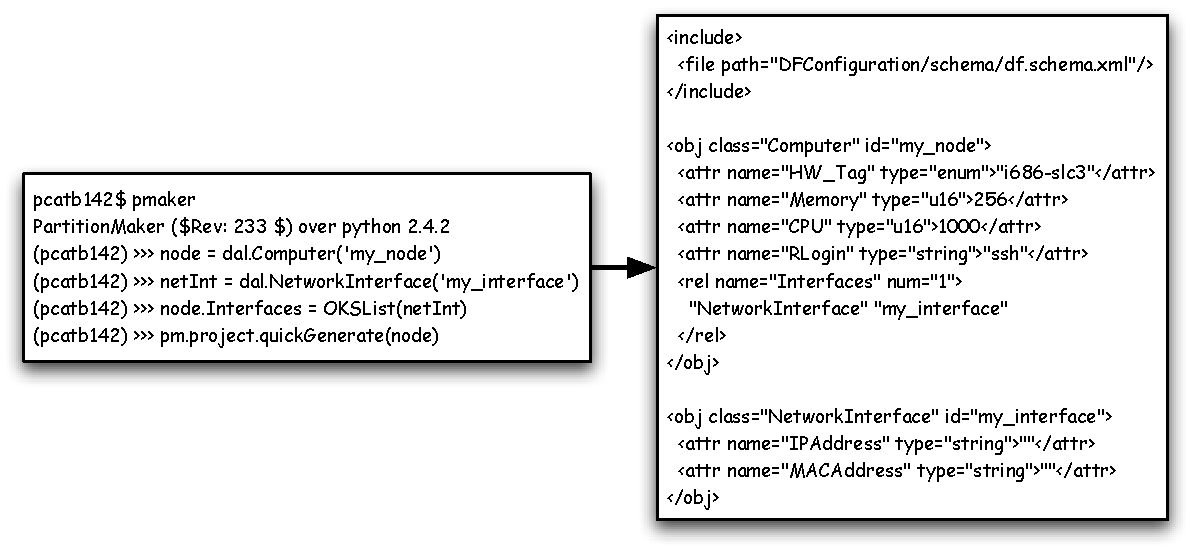
\includegraphics[width=0.7\textwidth]{ide}
\caption{Exemplo de geração de uma partição.}
\label{fig:ide}4
\end{center}
\end{figure}

É apresentado na Fig.~\ref{fig:pm_flow} um exemplo simplificado do fluxo de mensagens para a criação de uma partição contendo 8 ROS, além do LVL2 contendo 1 L2SV e 20 L2PU. No exemplo, o usuário trabalha somente com a camada mais alta. Ao especificar somente o número de componentes desejados, a camada de partição dispara mensagens para a camada de segmentos, de forma que sejam criados os segmentos para os ROS e LVL2. A camada de segmentos, por sua vez, ativa a camada de componentes, de forma que cada um dos objetos necessários sejam criados e retornados à camada de segmentos. Em seguida, a camada de segmentos agrupa tais componentes de maneira coerente à sua função, e os segmentos gerados são retornados para a camada de partição, para que sejam conectados e finalmente retornados ao usuário.

Outra etapa importante no processo de configuração é selecionar os nós de processamento a serem utilizados por cada aplicação. Para tal, o Módulo de Rastreamento de \emph{Hardware} permite rastrear um conjunto de máquinas de forma a analisar a propriedade destas (velocidade de \emph{clock}, quantidade de memória, interfaces de rede, etc), para melhor definir quais aplicações devem rodar em quais máquinas. Esta busca é feita em paralelo, através da utilização de várias \emph{threads} \cite{bib:modern_operating_systems} de execução, usando a estrutura de rede disponível. Isto resulta em tempos de busca bastante reduzidos, na ordem de poucas dezenas de segundos, para um conjunto de várias centenas de máquinas. 

Ao final deste processo de configuração, obtém-se uma representação da base de dados de configuração através de objetos em \emph{Python}. Esta base é então exportada, utilizando-se os recursos do módulo \emph{Projeto de Partição}, para o formato OKS de base de dados de configuração, podendo, finalmente, ser utilizada para a operação do sistema de filtragem de alto nível do ATLAS. Este módulo também permite que bases de dados de configuração já criadas possam ser importadas e editadas dentro do \emph{PartitionMaker}, proporcionando, desta maneira, que partições geradas com recursos externos ao \emph{PartitionMaker} também possam ser manipuladas neste ambiente.

Por ser implementado em \emph{Python}, o \emph{PartitionMaker} pode usufruir dos recursos bastante numerosos  desta linguagem. Como conseqüência, um ambiente integrado de desenvolvimento está disponível, permitindo rápida prototipagem de base de dados de configuração, conforme o exemplo na Fig.~\ref{fig:ide} demonstra. Ao inicializar o ambiente integrado, através do comando \texttt{pmaker}, o usuário acessa as funcionalidades do sistema. No exemplo, deseja-se configurar um nó de execução (\texttt{my\_node}) contendo uma interface de rede (\texttt{my\_interface}), usando, neste caso, a \emph{Camada de Componentes}. Ao final da configuração, os objetos criados em \emph{Python} são exportados para o formato utilizado pelo OKS através da função \texttt{quickGenerate}, cujo resultado aparece ao lado direito da Fig.~\ref{fig:ide}.

A facilidade da linguagem \emph{Python}, aliada ao ambiente integrado de desenvolvimento, permite que \emph{plugins} possam ser facilmente desenvolvidos para o \emph{PartitionMaker},  expandindo consideravelmente a capacidade do trabalho proposto. Por fim, como o ambiente integrado aceita comandos, tanto manualmente inseridos, bem como oriundos de um arquivo texto, \emph{scripts} de configuração podem ser escritos com facilidade, permitindo a execução de testes automáticos do sistema de filtragem do ATLAS, quando se deseja observar o comportamento deste sob diversas condições de operação (número de processadores, níveis de filtragem considerados, etc).

A abordagem utilizada para a concepção do \emph{PartitionMaker} resultou num claro aumento da produtividade dos desenvolvedores e operadores do sistema de filtragem do ATLAS. Antes, era necessária a presença de especialistas para garantir a correta configuração do sistema de filtragem. Com este conhecimento especialista embutido no \emph{PartitionMaker}, os usuários ficam mais independentes durante o processo de configuração. Isto resulta, também, em ganhos de produtividade para os técnicos especialistas, visto que minimiza-se a necessidade destes interromperem suas atividades para apoiar usuários menos experientes.

Outro resultado obtido foi a considerável diminuição de execuções mal sucedidas para os testes do sistema de filtragem do ATLAS. Com o \emph{PartitionMaker} identificando e notificando automaticamente possíveis erros durante a configuração, possíveis falhas podem ser identificadas antes da execução do sistema de filtragem, evitando-se a interrupção da operação do experimento.


\section{Automatic Online Triggering Execution}
\label{sec:runner}

Although the configuration process can be fully automated, by means of configuration database creation scripts, the execution of TDAQ is still manual. In order to start a given TDAQ run, once the configuration database is available, the following steps must be taken:

\begin{enumerate}

\item Boot: at this point the configuration database file is read, and the top level control applications are started. then, each control application starts up any controller placed beneath it within the segments hierarchy tree. After, each controller will start up any application within its segment, as well as all the configured RDB servers. All the applications are started up on the computer node designed for them in the database configuration file.

\item Configure: during this phase, the applications will retrieve their running configuration parameters from their RDB servers, which basically contain a cached copy of the original database configuration file. After this step, the TDAQ infrastructure is ready to begin its operation.

\item Run: this is the phase where data is actually being read from ATLAS detectors for the nominal use case, or from Monte Carlo simulation files if the TDAQ execution is envisaged for testing purposes. During this step, monitoring applications samples all TDAQ resources (memory consumption, LVL1 accept rate, CPU utilization, etc.), they also generate online histogramming with timing information, decision threshold achieved, etc. Finally, log files are created on the application nodes with any useful information for posterior analysis (warning / error messages issued, etc.). This running state is sustained until explicit user intervention requiring its interruption.

\end{enumerate}

While issuing the commands above manually is reasonable for the nominal operation case, it is quite tedious to perform all theses steps manually when several testing cases must be covered, which is a common case in the TDAQ development, either for TDAQ new releases validation and overnight tests, as well as for validation of new acquired hardware.

\begin{figure}
\begin{center}
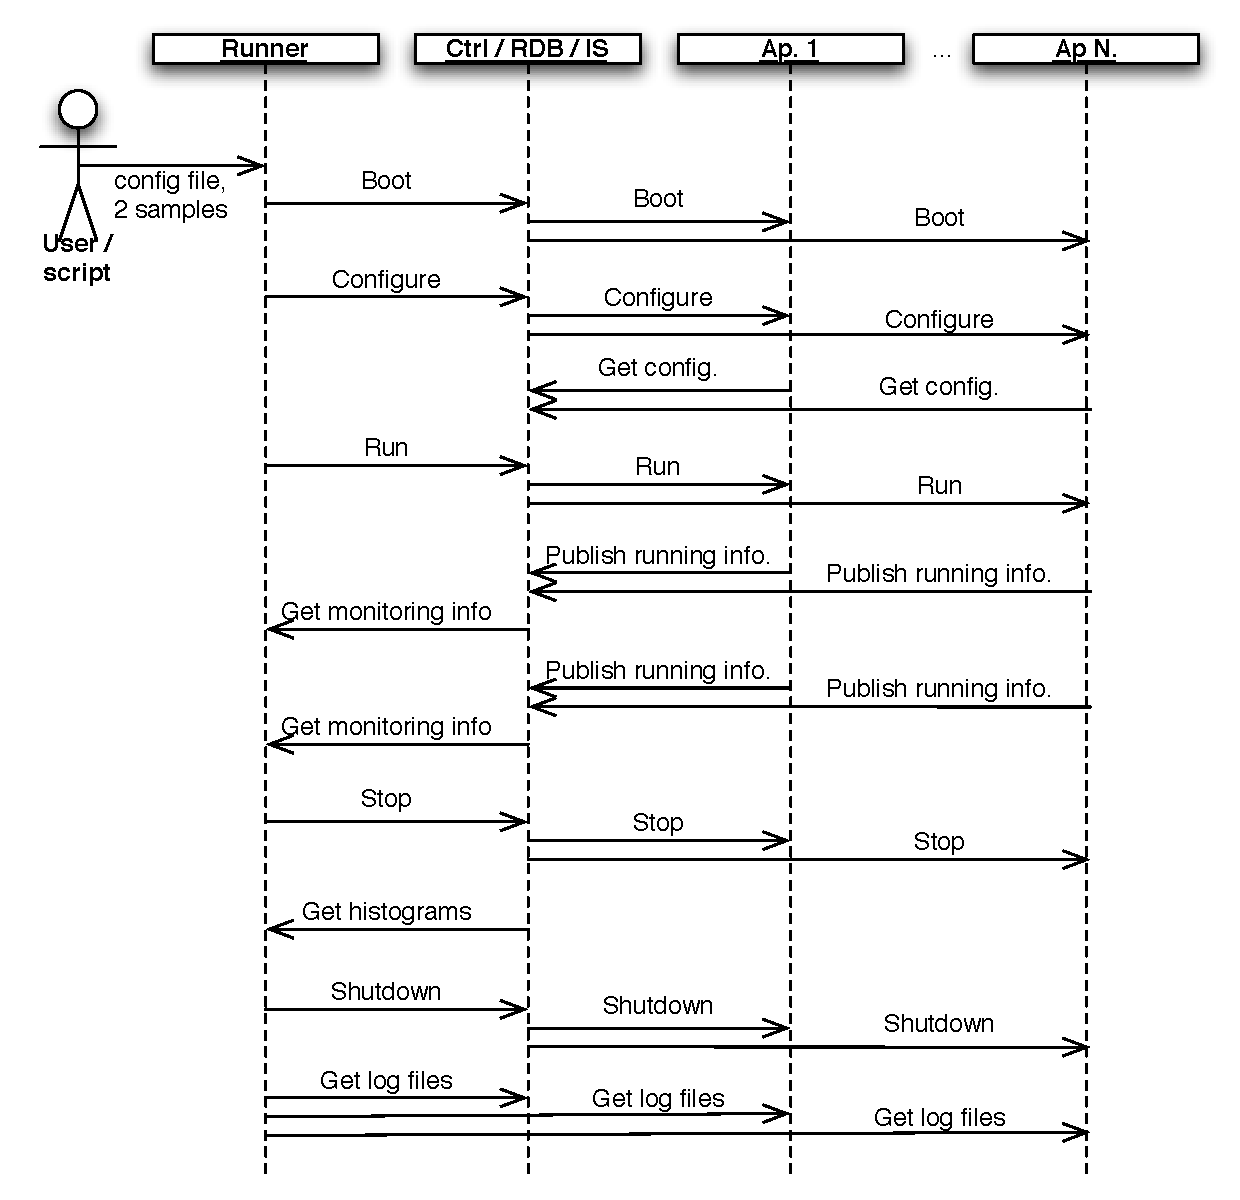
\includegraphics[width=0.6\textwidth]{runner_execution_flow}
\end{center}
\caption{Runner execution flow example.}
\label{fig:runner_exec_flow}
\end{figure}

Having this necessity in mind, the \emph{Runner} environment was developed. Its main goal is to provide an automated / scriptable way of running the TDAQ infrastructure, as well as collecting its monitoring information from the monitoring applications providing, if desired, a summarized report of the overall TDAQ execution. In Fig.~\ref{fig:runner_exec_flow} is presented a general example of the \emph{Runner} execution flow. In this example, the user (a running script, for instance) provides the configuration database file, and requests the TDAQ infrastructure to be executed for a time long enough so that 2 monitoring samples can be obtained. First the \emph{Runner} sends the message to the controller to boot the TDAQ modules to be used for this particular run. The controller then propagates the boot command to the rest of the applications. Next, the same sequence takes place, but this time to ask each TDAQ application to retrieve their configuration from the RDB server. In the next step, the \emph{Runner} asks the controller to send the command to start TDAQ operation. After that, each application will publish their monitoring information on their IS server, which is the application responsible for storing monitoring information. By knowing the monitoring sampling period, the \emph{Runner} can request the monitoring information published on the IS server. In the mean time, the online histogramming are being filled by the IS server. Once the 2 monitoring samples are collected, the \emph{Runner} issues the stop command to the controller, which propagates the command to all TDAQ applications. After, the online histograms are retrieved from the IS server, and the TDAQ infrastructure is requested to be shutdown. After this step, the \emph{Runner} connects to each of the nodes used in this TDAQ run to collect their log files. At the end, the monitoring information, log files and online histograms are returned to the user for further analysis, if desired.

The \emph{Runner} is presented as a set of Python modules. Therefore, the same IDE and syntax language available for the \emph{PartitionMaker} are available for the \emph{Runner}.  Consequently, plugins and running scripts can be easily developed for this environment. By combining these 2 environments, with an analysis framework with a Python interface, like ROOT \cite{bib:root}, the configuration, execution and analysis of the data obtained during TDAQ execution can be fully automated, greatly improving validation capabilities of the overall TDAQ infrastructure.


